\documentclass{article}
\usepackage[utf8]{inputenc}
\usepackage{amsmath, esint}
\usepackage{wasysym}
\usepackage[colorlinks]{hyperref}
\usepackage{lmodern}
\usepackage{graphicx}
\usepackage{xcolor}
\usepackage[left=2cm, top=3cm, right=2cm]{geometry}
\usepackage{minted}
\usepackage{xcolor}
\definecolor{LightGray}{gray}{0.975}

%setup new colors
\hypersetup{
%linkcolor=blue
%,citecolor=
%,filecolor=
urlcolor=blue
%,menucolor=
%,runcolor=
%,linkbordercolor=
%,citebordercolor=
%,filebordercolor=
%,urlbordercolor=
%,menubordercolor=
%,runbordercolor=
}

\title{Databases\\Lab 03}
\author{Andrés Calderón, Ph.D.}
\date{\today}

\begin{document}

\maketitle

\section{Introduction}
We will work in three parts today.  First, we will reinforce what we learn in class watching a couple of videos from \href{https://www.w3schools.com/}{w3schools.com} about basic SQL.  Then we will explore some of the lessons in the interactive tutorial from the same website.  Finally, we will finish running some SQL code in the \texttt{university} database we will download from the book website.

Let's go!

\section{W3Schools SQL YouTube Videos}
We will watch a YouTube playlist from the w3shools.com channel about introductory SQL.  You can access the playlist \href{https://youtu.be/zpnHsWOy0RY?si=Lo7BQJ9PNjVmOsW4}{here}.  You can activate the Spanish subtitle in the Settings button if you want.  There are 11 short videos.  Just watch them, there are not any particular submission to do for now.

\section{W3Schools Interactive SQL Tutorial}
Now, you will go through the interactive SQL tutorial at the W3Schools website, so first you need to create an account.  The tutorial start \href{https://www.w3schools.com/sql/}{here}.  You will see several lessons in the left panel (red square in Figure \ref{fig:panel}).  You only have to cover the followings:

\begin{itemize}
  \item Intro
  \item Syntax
  \item Select
  \item Select Distinct
  \item Where
  \item Order By
  \item And
  \item Or
  \item Not
  \item Null Values
  \item Aggregate Functions
  \item Min and Max
  \item Count
  \item Sum
  \item Avg
  \item Like
  \item Wildcards
  \item In
  \item Between
  \item Aliases
\end{itemize}

Remember capture and screenshot when you execute each of the SQL statement so you can attach them later on your report.  Try to capture your username if possible.

\begin{figure}[t]
 \centering
 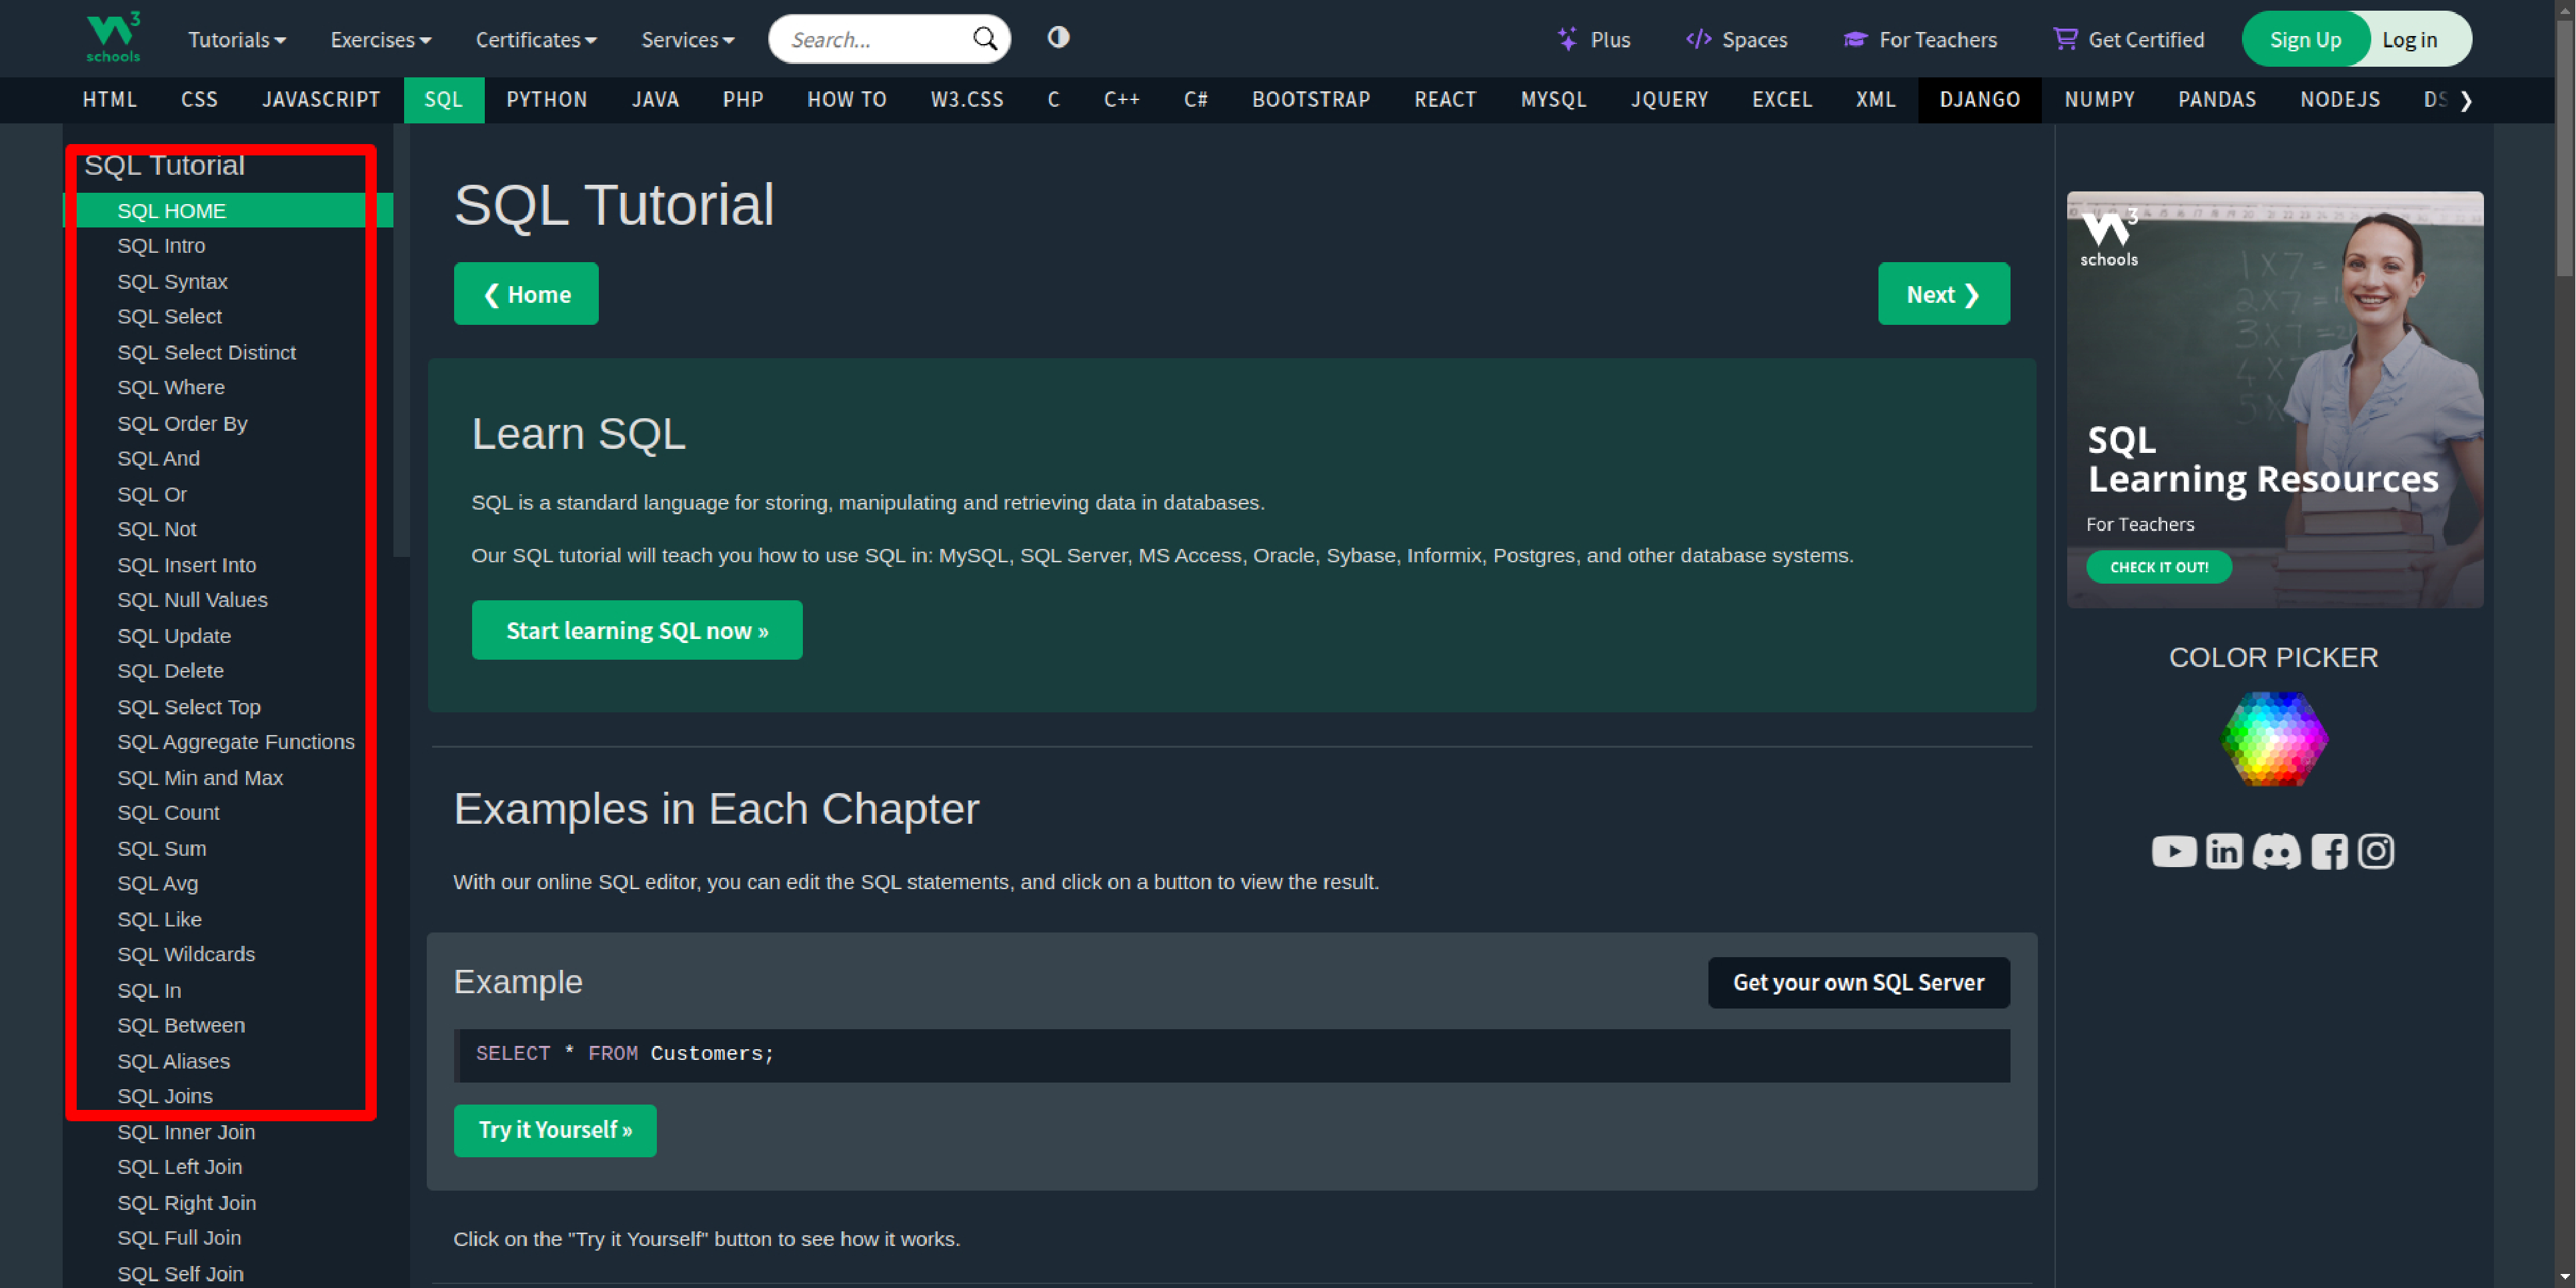
\includegraphics[width=\textwidth]{figures/panel}
 \caption{Lessons panel at W3Schools SQL Tutorial.}
 \label{fig:panel}
\end{figure}

\section{The \texttt{university} Database}
The webside of the book \textit{``Database System Concepts''} provides backups of the \texttt{university} database we have been following in classes.  We will load a small version in PostgreSQL so we can practice a bit the SQL statements we already saw.  You will need to download two files:

\begin{enumerate}
  \item The \href{https://db-book.com/university-lab-dir/sample_tables-dir/DDL.sql}{\texttt{DDL.sql}} file with the code to create the database structure.
  \item The \href{https://db-book.com/university-lab-dir/sample_tables-dir/smallRelations/smallRelationsInsertFile.sql} {\texttt{smallRelationsInsertFile.sql}} file with the code to populate the database with the same records we can find in the book examples.
\end{enumerate}

Download both files at put them in the same folder.

We will assume that you have already a functional instance of PostgreSQL running in your machine.  We expect you have access to a PostgreSQL console similar that Figure \ref{fig:psql}.

\begin{figure}[h]
 \centering
 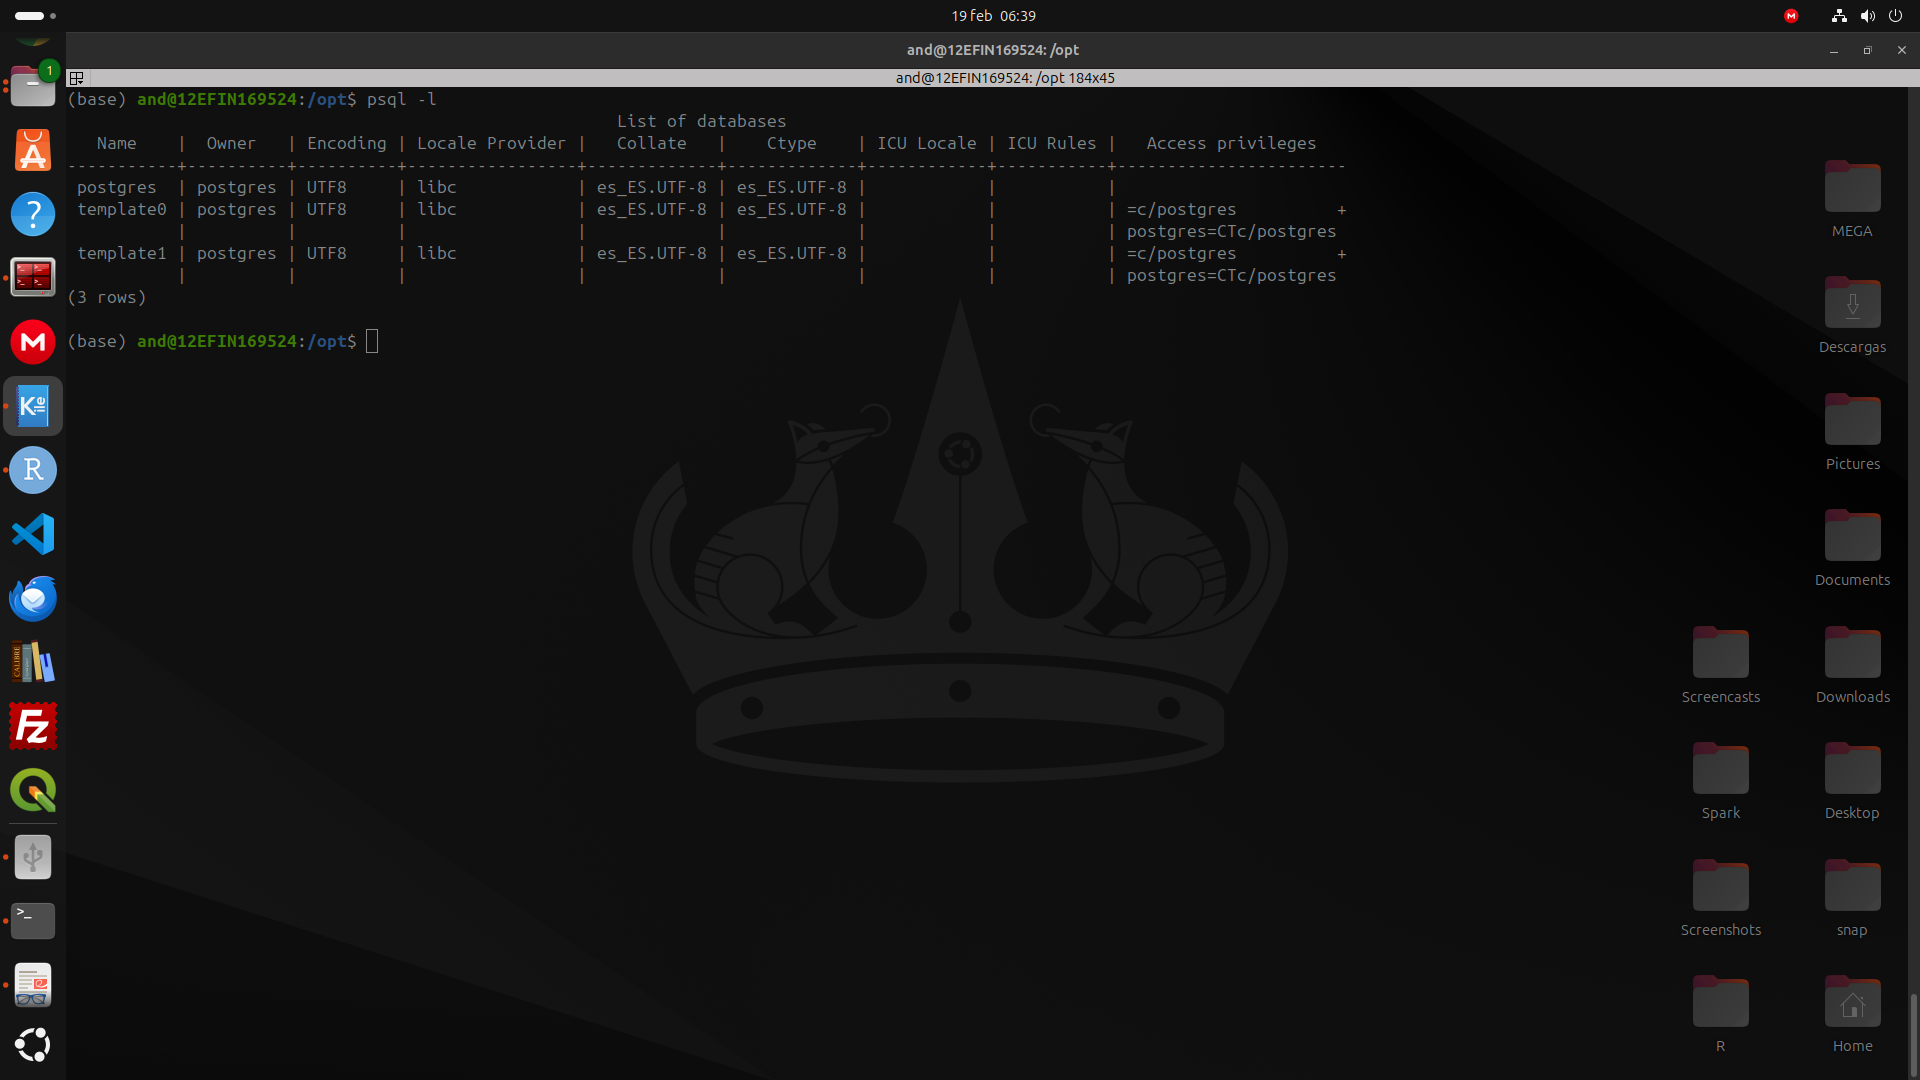
\includegraphics[width=\textwidth]{figures/psql}
 \caption{PostgreSQL installed in your system.}
 \label{fig:psql}
\end{figure}

First, we will create a database named \texttt{university}:

\begin{minted}
[tabsize=4, obeytabs, frame=lines, framesep=2mm, baselinestretch=1.2, bgcolor=LightGray, fontsize=\footnotesize]{bash}
createdb university
\end{minted}

Next, we will connect to that database:
\begin{minted}
[tabsize=4, obeytabs, frame=lines, framesep=2mm, baselinestretch=1.2, bgcolor=LightGray, fontsize=\footnotesize]{bash}
psql university
\end{minted}

Now we are in the PostgreSQL prompt.  There we will use the \textbackslash i command to load the schema and data for our database.  You will need to change the paths of the downloaded files accordingly.

First, we load the \texttt{DDL.sql} file:
\begin{minted}
[tabsize=4, obeytabs, frame=lines, framesep=2mm, baselinestretch=1.2, bgcolor=LightGray, fontsize=\footnotesize]{bash}
\i /path_to_files/DDL.sql
\end{minted}

Then, the \texttt{smallRelationsInsertFile.sql} file:
\begin{minted}
[tabsize=4, obeytabs, frame=lines, framesep=2mm, baselinestretch=1.2, bgcolor=LightGray, fontsize=\footnotesize]{bash}
\i /path_to_files/smallRelationsInsertFile.file
\end{minted}

And you are done!  Let's try some SQL:
\begin{minted}
[tabsize=4, obeytabs, frame=lines, framesep=2mm, baselinestretch=1.2, bgcolor=LightGray, fontsize=\footnotesize]{sql}
SELECT * FROM instructor;
\end{minted}

Now you are ready to explore the SQL we have already seen in class.

\section{Independent Work}
Now that we have the \texttt{university} database ready to go, you are asked to answer the following queries:

\begin{enumerate}
  \item Retrieve the names of all instructors, along with their department names and department building name.
  \item For all instructors in the university who have taught some course, find their names and the course ID of all courses they taught.
  \item Find the names of all departments whose building name includes the substring `Watson'.
  \item Find the set of all courses taught in the Spring 2018 semester and in the Fall 2017 semester.
  \item Find all instructors who appear in the instructor relation with null values for salary.
  \item Find the average salary in each department.
  \item Show those departments where the average salary of the instructors is more than \$42,000.
  \item Find the total number of (distinct) students who have taken course sections taught by the instructor with ID 110011.
  \item Find the names of all instructors that have a salary value greater than that of each instructor in the Biology department.
  \item Finally you will propose your own query and solve it using SQL by you own.
\end{enumerate}


For each query you have to present its corresponding Relational Algebra Expression, the SQL code, and the result of the query (copy-paste or screenshot).
We expect you to submit a well-structured report in PDF format, containing the requested information in the previous sections. Additionally, include the \texttt{SQL} code with the answers to the queries in a ZIP file. The submission deadline is \textbf{March 5th, 2025}.

\vspace{4mm}
Happy Hacking \smiley!


\end{document}
